\chapter{Anexo}

\section{Glosario de movimientos}

%\begin{minipage}{0.5\textwidth}
\begin{table}[h]
\resizebox{\textwidth}{!}{%
\centering
\label{glosario}
\begin{tabular}{lll}
\toprule
{} &                         Significado &                          Traducción \\
\midrule
thruster          &                            Thruster &                            Thruster \\
chest-to-bar      &                Chest-to-bar pull-up &                   Dominada al pecho \\
double-unders     &              Double-under rope jump &                Salto doble de comba \\
ghd               &  Glute-ham developer machine sit-up &          Abdominales en máquina GHD \\
power clean       &                         Power clean &                   Cargada de fuerza \\
deadlift          &                            Deadlift &                         Peso muerto \\
shspu             &            Strict handstand push-up &            Flexión de pino estricta \\
ohs               &                      Overhead squat &             Sentadilla de arrancada \\
bar-facing burpee &                   Bar-facing burpee &  Burpee frente a la barra con salto \\
\bottomrule
\end{tabular}
}
\end{table}
%\end{minipage}


\section{Probabilidades obtenidas por movimiento en la muestra de test}\label{Probabilidades}

En la siguiente imagen se puede observar, para cada movimiento observado, las probabilidades que devuelve el modelo.

Si nos fijamos en la imagen \textit{ohs vs rest} por ejemplo, podemos ver los movimientos entre las probabilidades que dan pie a las figuras de los heatmap de las correlaciones, figura \ref{heatmap_correlations}, donde se puede observar como cuando disminuye probabilidad de \textit{ohs}, aumenta la probabilidad de \textit{thruster}.

\begin{figure}[H]
    \centering
		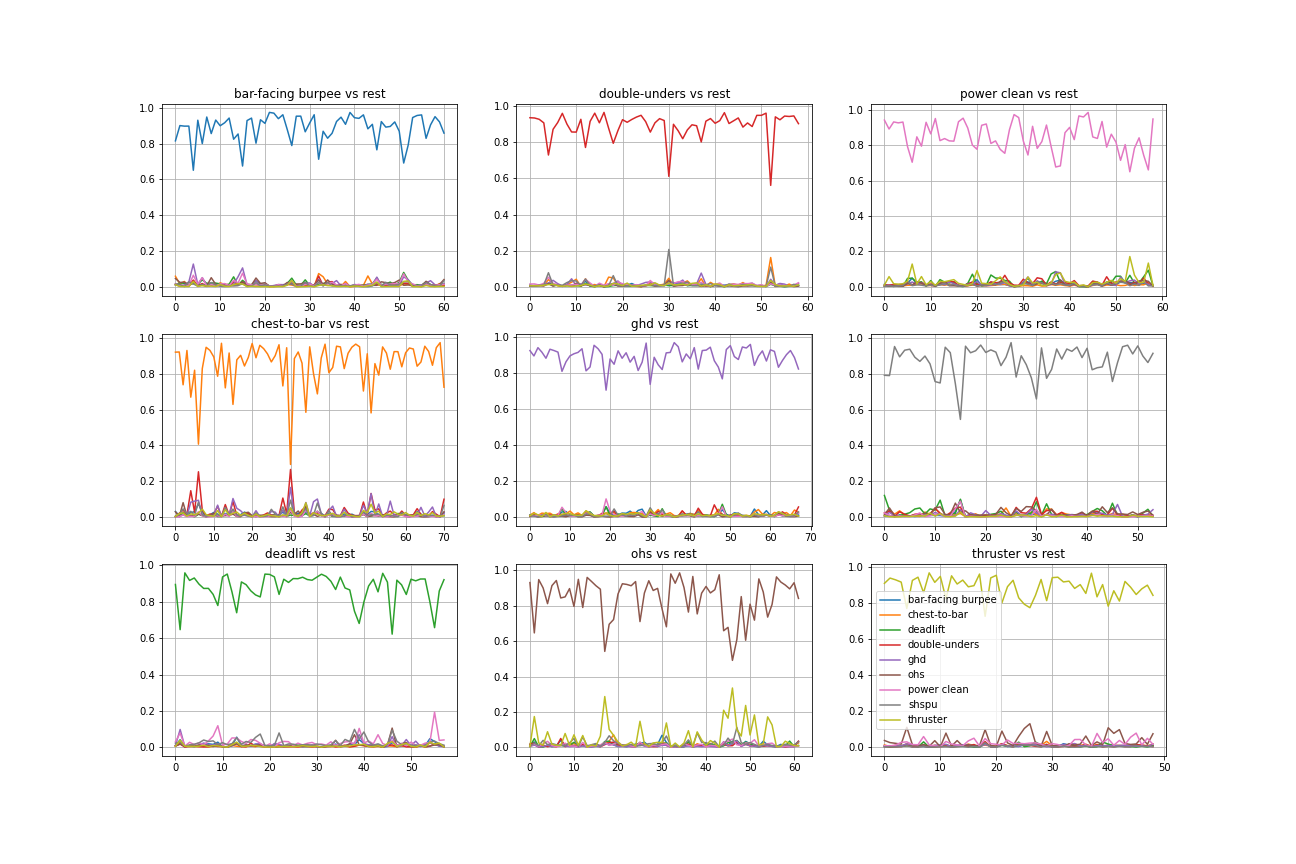
\includegraphics[width=\textwidth]{figs/probabilities_by_movement.png}
\caption{Probabilidad estimadas en la muestra de test. Para cada movimiento observado, cada gráfica representa las probabilidades obtenidas por el modelo.}\label{probabilities_by_movement}
\end{figure}



\section{Pipeline en AWS}

A la hora de tratar los videos en la función lambda hay que tener en cuenta lo siguiente, si se parte de la imagen de docker que ofrece \href{https://hub.docker.com/r/amazon/aws-lambda-python}{AWS} (como es el caso). Para leer los videos en mp4 y traducirlos a tensores para que los pueda entender tensorflow, se ha utilizado la siguiente función: \href{https://www.tensorflow.org/io/api_docs/python/tfio/experimental/ffmpeg/decode_video}{decode\_video}. Esta función parte de unos binarios que fallan en la distribución de linux que utiliza la imagen de docker, ver \href{https://github.com/tensorflow/io/issues/1648}{issue}. Como alternativa para leer los videos en este caso se ha utilizado \href{https://pypi.org/project/opencv-python-headless/}{OpenCV}, si bien el impacto impacto que tiene es mínimo a la hora de leer los clips, en los decimales usados al pasarlo a tensor.
